\Chapter{Koordináta-rendszerek}

\section{Négyzet alapú rendszerek}

A négyzet alapú koordináta-rendszer alatt jelen esetben a hagyományos \textit{Descartes-féle} koordináta-rendszert értjük. Ennek a pontjait az $(x, y) \in \mathbb{Z}^2$ alakban írhatjuk föl.

% "A síkbeli \textit{Descartes-féle koordináta-rendszer}ben egy $P$ pont helyzetét az $XY$ síkon az $(x;y)$ rendezett számpárral (koordináta-kettős) adjuk meg. A két tengely metszéspontja a koordináta-rendszer kezdőpontja az origó $(O)$. A megállapodás szerinti első $x$ koordináta az abszcissza, a második $y$ koordináta az ordináta. Ugyanezekkel a jelzőkkel különböztetjük meg a tengelyeket. A vektoros értelmezésnél az $X$ és $Y$ tengelyek irányába mutató egységvektorokat $(i;j)$ jelöli." \cite{WikiSquare}

\section{Hexagon alapú rendszerek}
\label{sec:hexagon}

A hexagonok hat oldalú poligonok. A szabályos hatszögnek minden oldala egyenlő hosszúságú és belső szögei is egyenlőek. A szakdolgozatomban olyan hexagonokkal foglalkozok, amelyeknek a szemközti oldalai egyenlő hosszúságúak és párhuzamosak, viszont nem minden esetben feltétlenül szabályosak \cite{HexWiki}.

Egy hexagonnak hat oldala van. Minden oldalon két hexagon osztozik. Egy hexagonnak hat csúcsa van, minden csúcson 3 hexagon osztozik. A hexagonháló esetében többfajta megközelítés is szóbajöhet, most ezek közül fogok néhányat ismertetni.

A hexagonokból felépülő rácsokban a koordináták kezelésére többféle módszer is adódik. A következő szakaszokban ezeket veszem sorra, és hasonlítom össze.

\subsection{Eltolásos koordináta-rendszer}
% \cite{redblobgamesHexagonalGrids}

A leggyakoribb megközelítés a hexagon alapú rácsokban lévő koordináták kezeléséhez az eltolásos módszer, ami kisebb eltérésektől eltekintve gyakorlatilag megegyezik a \textit{négyzet koordináta-rendszer}rel. A \textit{négyzet koordináta-rendszer}hez hasonlóan itt is a hálónk egyik sarka lesz a kezdő pont (origó) amihez viszonyítva számozzuk majd a sorokat és az oszlopokat.

Az \textit{eltolásos koordináta-rendszer} egyik hátránya, hogy az egyik tengelye mentén nem egyenesen haladnak a sokszögek az eltolás miatt, és emiatt bonyolultabbá válnak a számítások (\ref{fig:OffsetCoord}. ábra). A további rendszerek ezt a problémát orvosolják, viszont ott más nehézségek merülnek fel.	

\begin{figure}[h!]
\centering
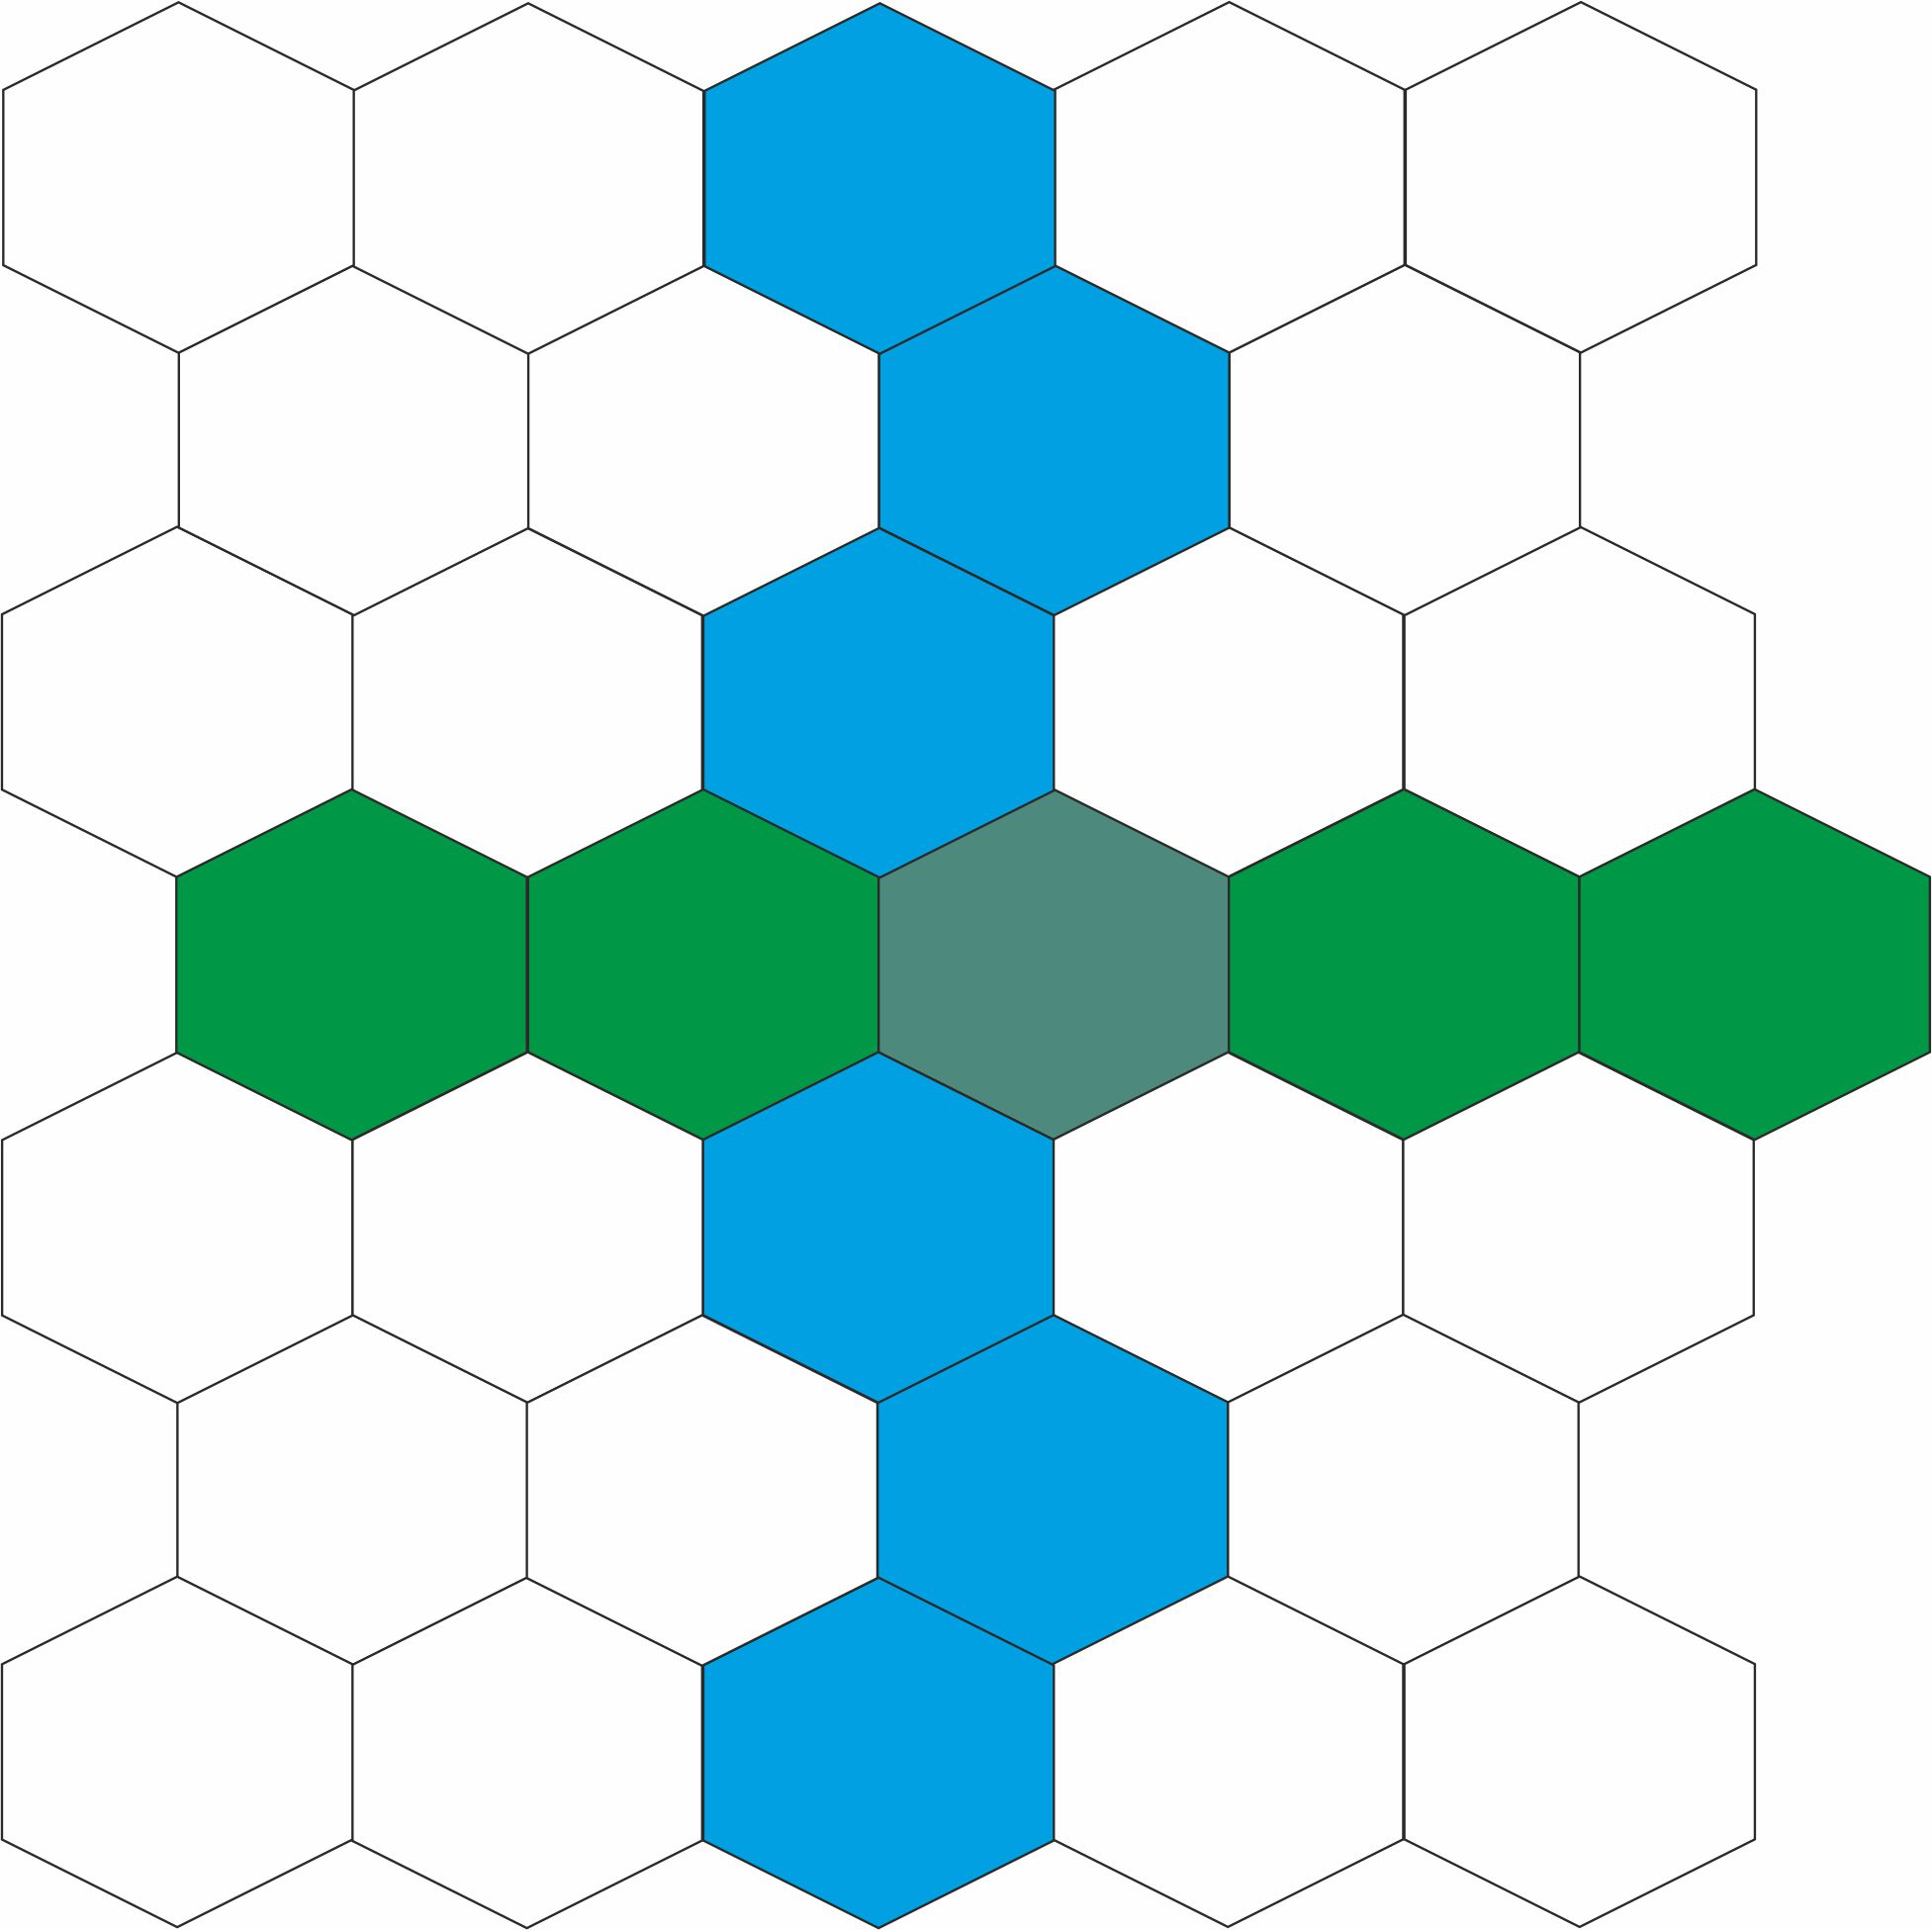
\includegraphics[scale=0.3]{kepek/OffsetCoord.jpg}
\caption{\textit{Eltolásos koordináta-rendszer}ben a tengelyek elhelyezkedése}
\label{fig:OffsetCoord}
\end{figure}

\newpage
A négyzethálóval is elérhetünk a hexagonhálóhoz hasonló hatást, ha a négyzethálóban minden páros/páratlan sort/oszlopot eltolunk (\ref{fig:Hex_Sq}. ábra).

\begin{figure}[h!]
\centering
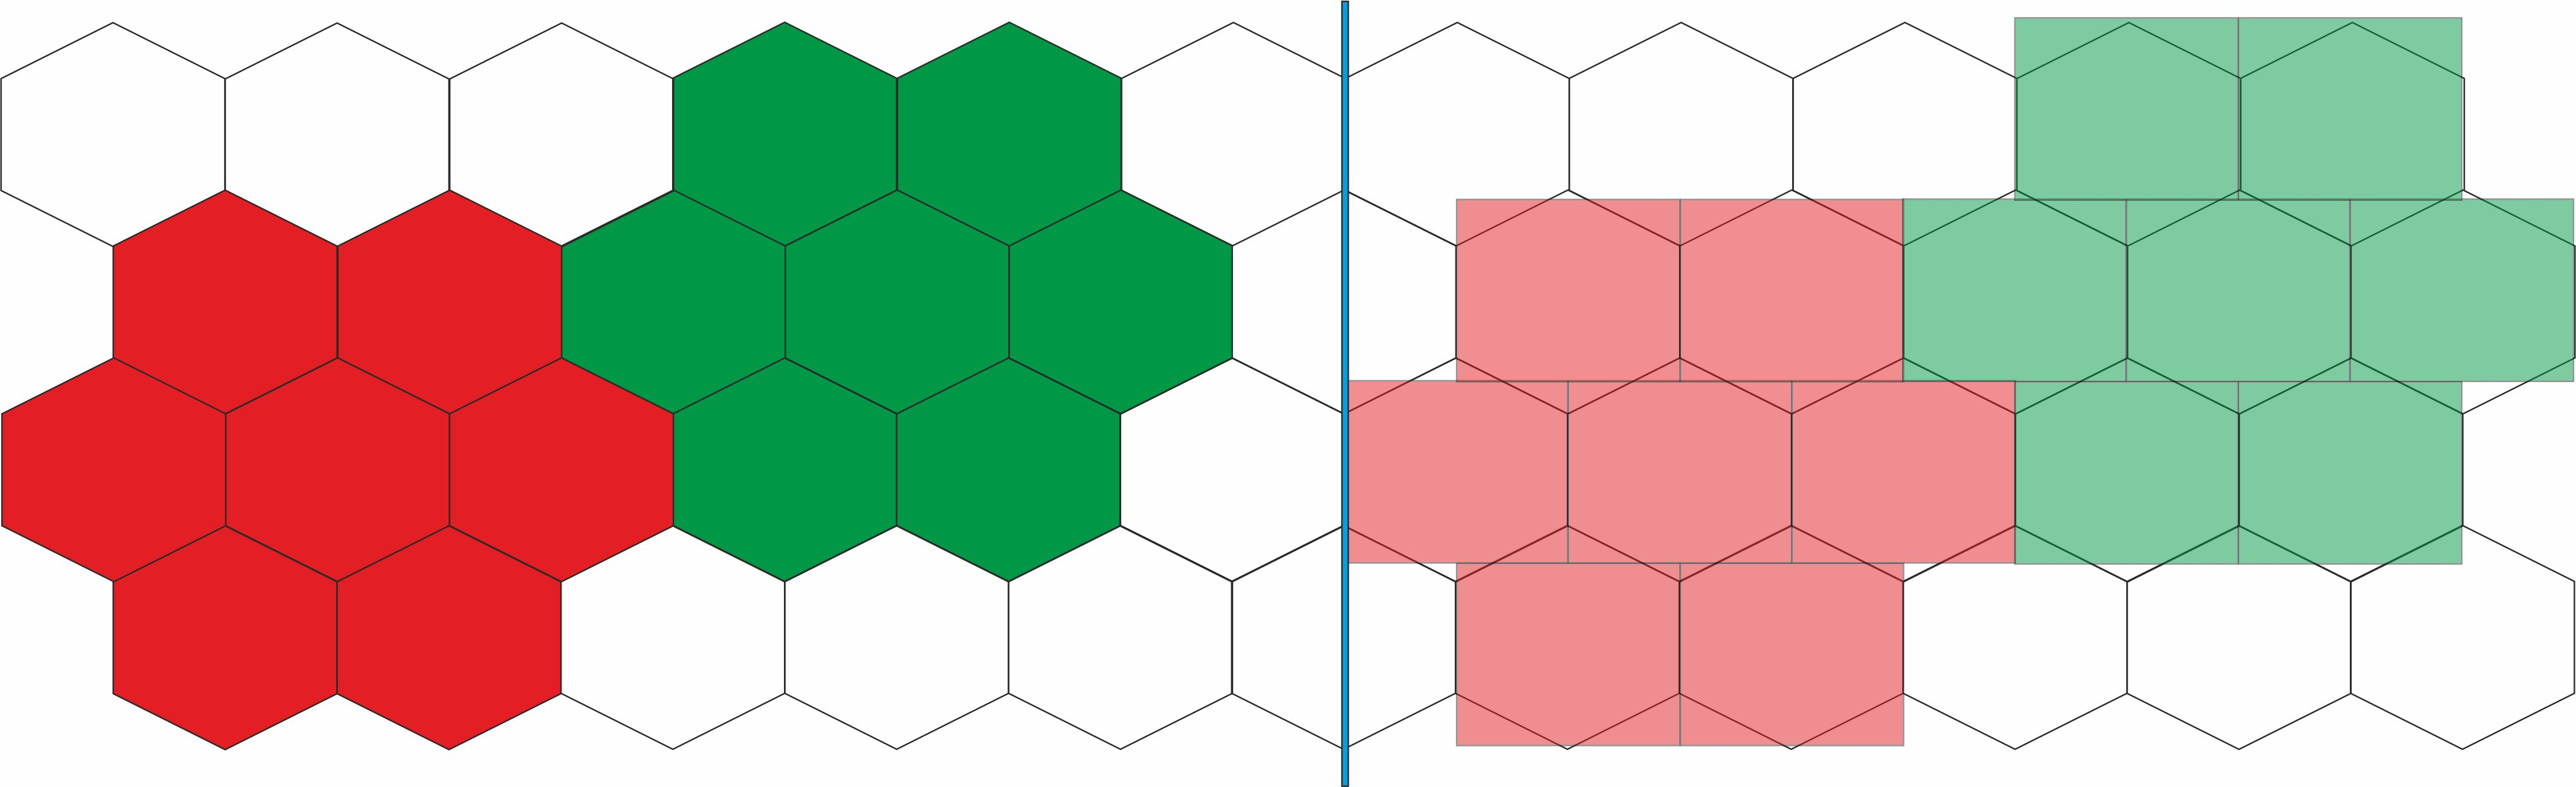
\includegraphics[scale=0.3]{kepek/Hex_Sq.jpg}
\caption{Hexagonrács az eltolt négyzetrácshoz viszonyítva}
\label{fig:Hex_Sq}
\end{figure}

Eltolható a páros és a páratlan oszlop/sor is. Mivel kétféleképpen is állhatnak a hexagonok, ezért négy fajta variáció érhető el összesen (\ref{fig:OffsetFour}. ábra) \cite{Offset}.

\begin{figure}[h!]
\centering
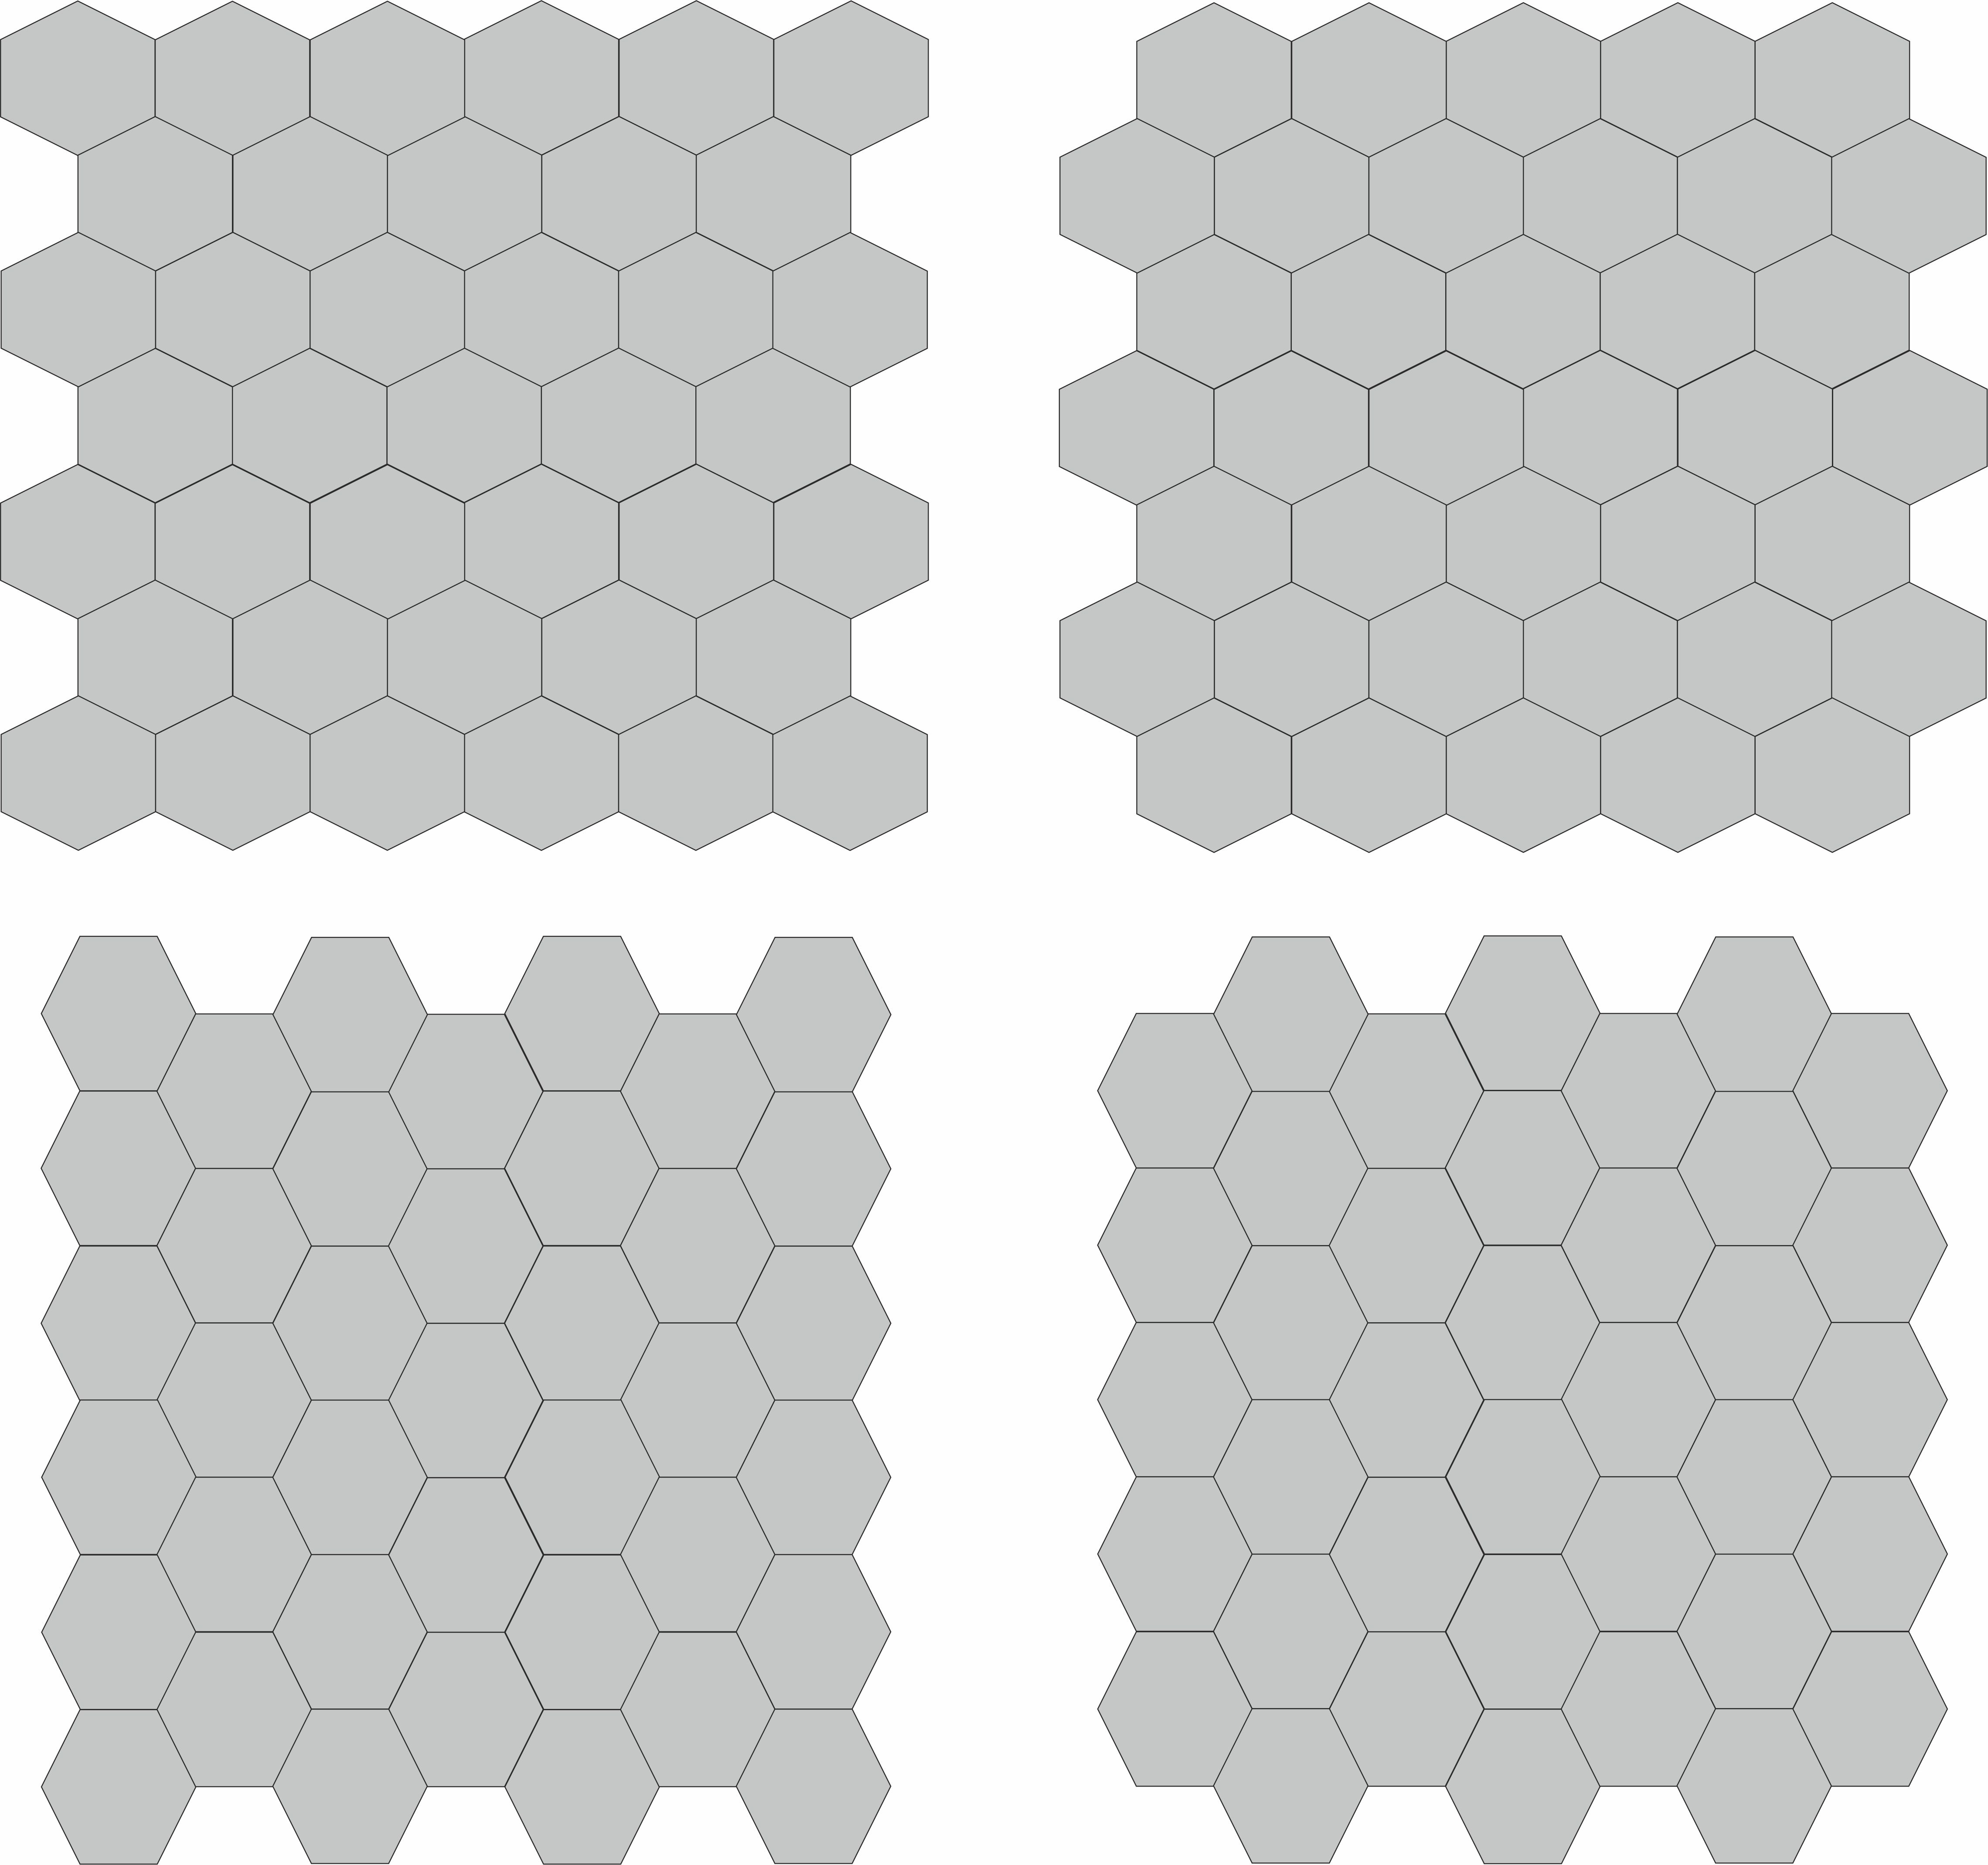
\includegraphics[scale=0.2]{kepek/OffsetFour.jpg}
\caption{A négyféle ábrázolási mód}
\label{fig:OffsetFour}
\end{figure}

\newpage
\subsection{Kocka koordináta-rendszer}
%\cite{redblobgamesHexagonalGrids}

Ha egy másik fajta megközelítésből nézzük a hexagon hálókat, akkor láthatjuk, hogy három elsődleges tengelye van, nem úgy mint a korábbi koordináta-rendszereknek (\ref{fig:CubeCoord}. ábra).

\begin{figure}[h!]
\centering
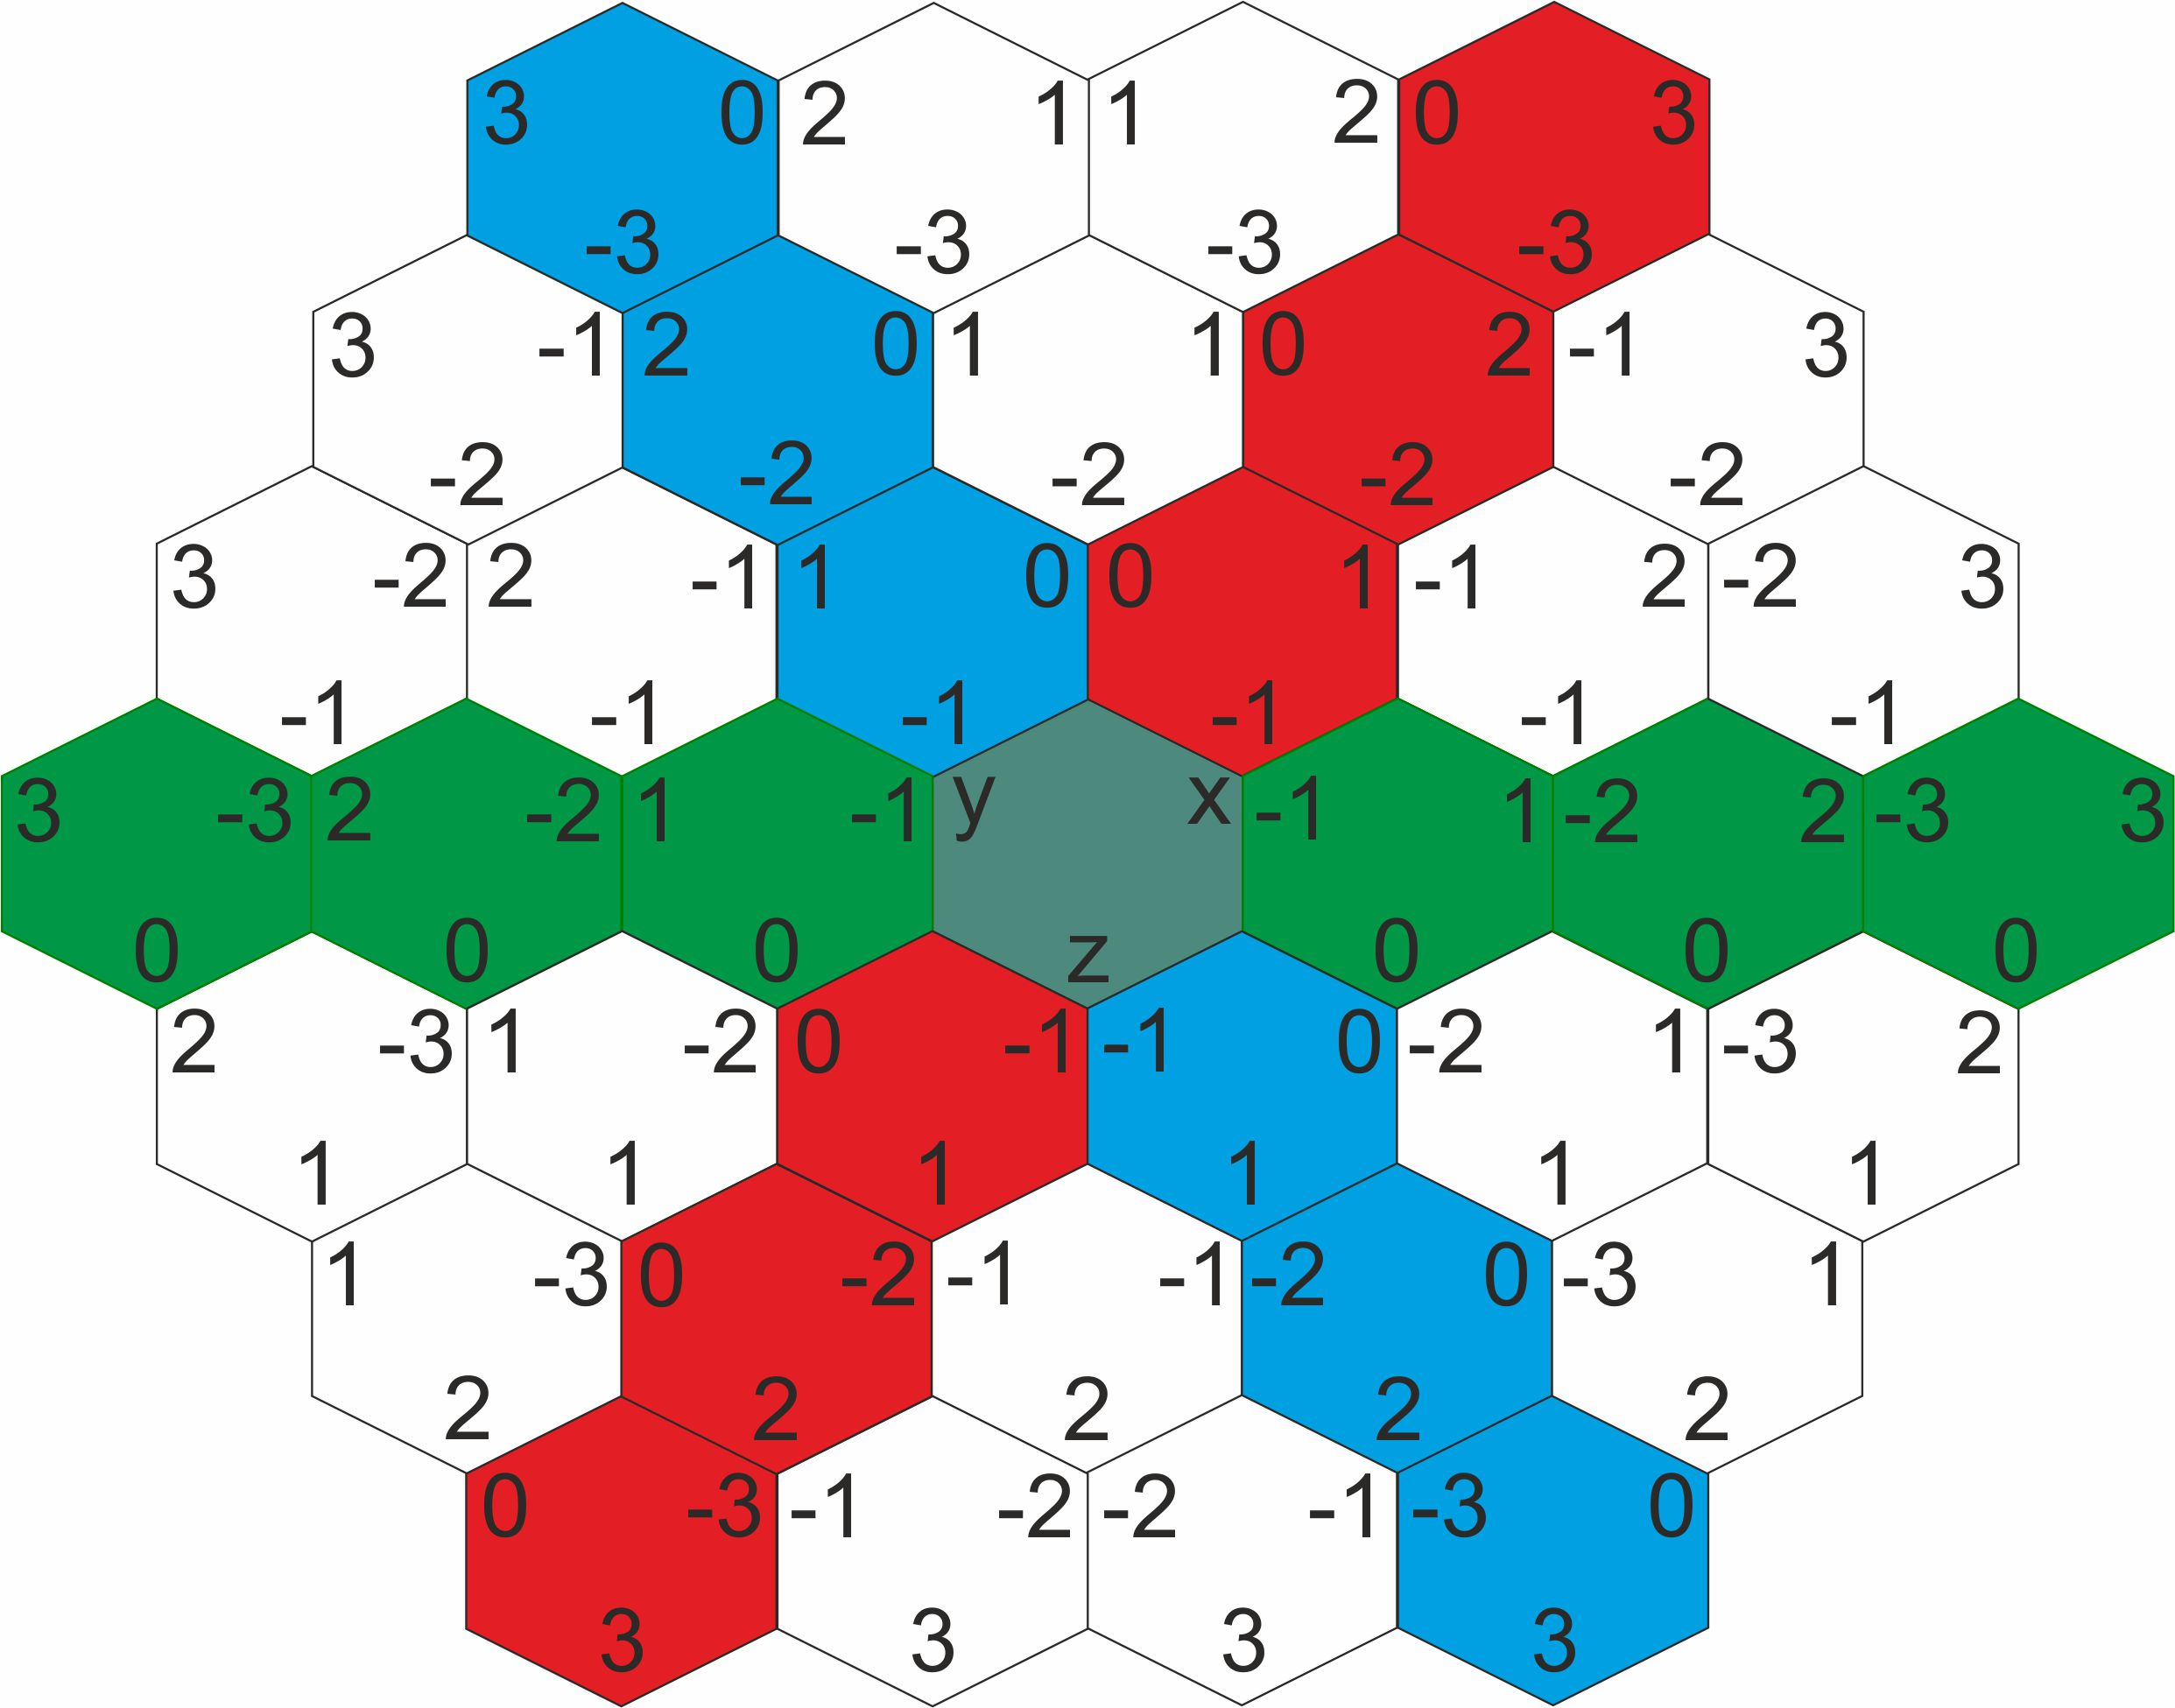
\includegraphics[scale=0.4]{kepek/CubeCoord.jpg}
\caption{A \textit{kocka koordináta-rendszer}ben a tengelyek elhelyezkedése}
\label{fig:CubeCoord}
\end{figure}

Ahhoz, hogy megértsük a \textit{kocka koordináta-rendszer}t képzeljünk el egy kockarácsot és vágjunk ki belőle egy átlós síkot az $x + y + z = 0$ mentén. Ez fogja majd a hexagonrácson használt algoritmusokat egyszerűbbé tenni azáltal, hogy használhatjuk a \textit{Descartes-féle koordináta-rendszer}ben való műveleteket. Ilyen műveletek az eltolás hozzáadása vagy kivonása a  koordinátákból, szorzás vagy osztás skalárral, távolság számítása.

Egy szemléletesebb példaként vizsgáljuk meg a \textit{Q*bert} nevű játékot (\ref{fig:Qbert}. ábra).

\begin{figure}[h!]
\centering
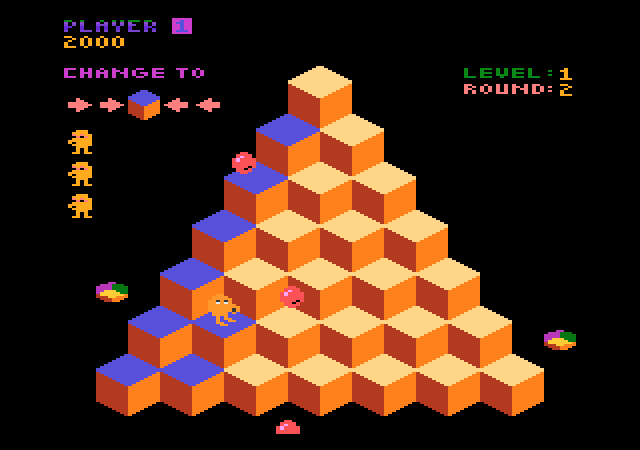
\includegraphics[scale=0.5]{kepek/Qbert.png}
\caption{A \textit{Q*bert} című játék}
\label{fig:Qbert}
\end{figure}

A játék egy $28$ kockából álló, piramis szerű játékmezőn zajlik. (Ilyen alakzatot kapunk, ha végrehajtjuk az előző részben leírt síkkal való vágást.) \newpage \noindent A játékos \textit{Q*bert}-et (narancssárga karakter) irányítja, aki, ha ráugrik egy kockára akkor átszínezi azt. Ha jobban megfigyeljük az ábrát, akkor láthatjuk, hogy a kockák valójában hexagonok, ha síkba rajzoljuk le. Így tehát \textit{Q*bert} 6 különböző irányba is léphet. Ez azt jelenti, hogy ha a párhuzamosan lévő oldalakra merőlegesen helyezünk tengelyeket, akkor hármat tudunk elhelyezni 120 fokonként. Vegyük észre az alábbiakat \cite{HexagonalGrids}.
\begin{itemize}
\item Minden hexagonnak 3 koordinátája van. 
\item Mindegyik tengely egy egyenes vonalnak felel meg a hexagon hálón.
\item Minden irány a hexagonon másik két iránynak a kombinációja a \textit{kocka koordináta-rendszer}en. Például, ha a \ref{fig:Qbert}. ábrán felfelé szeretnénk mozogni, akkor az a $+y$ és $-z$ között fekszik, ezért minden lépésnél ami felfelé történik hozzá kell adnunk 1-et az $y$-hoz és el kell vennünk 1-et a $z$-ből. 
\end{itemize}
Ez azért történik így, mert minden egyes mező koordinátájának az összege $0$ kell, hogy legyen ($x + y + z = 0$). Ez azt is jelenti, hogy a harmadik tengely bizonyos esetekben redundáns is lehet, például amikor meghatározzuk, hogy az egyes mezők hol jelenjenek meg a képernyőn. Ugyanakkor olyan esetekben amikor algoritmusokat (útkereső algoritmus) kell használni az előnye egyértelműen látszik (az algoritmusok könnyebb használhatósága miatt) \cite{Cube}. 

\subsection{Tengely koordináta-rendszer}

A \textit{tengely koordináta-rendszer} csak két koordinátát használ a \textit{kocka koordináta-rendszer} három koordinátája közül (\ref{fig:AxialCoord}. ábra). Mivel a \textit{kocka koordináta-rendszer}nél szükségszerű, hogy  $x + y + z = 0$ teljesüljön, a harmadik koordináta redundáns.  A \textit{tengelyes koordináta-rendszer} használható tárolásra és megjelenítésre, mivel az $x + y + z = 0$ egyenlet alapján kiszámítható a harmadik koordináta ezért a számításokhoz is könnyen használható \cite{Axial}.

\begin{figure}[h!]
\centering
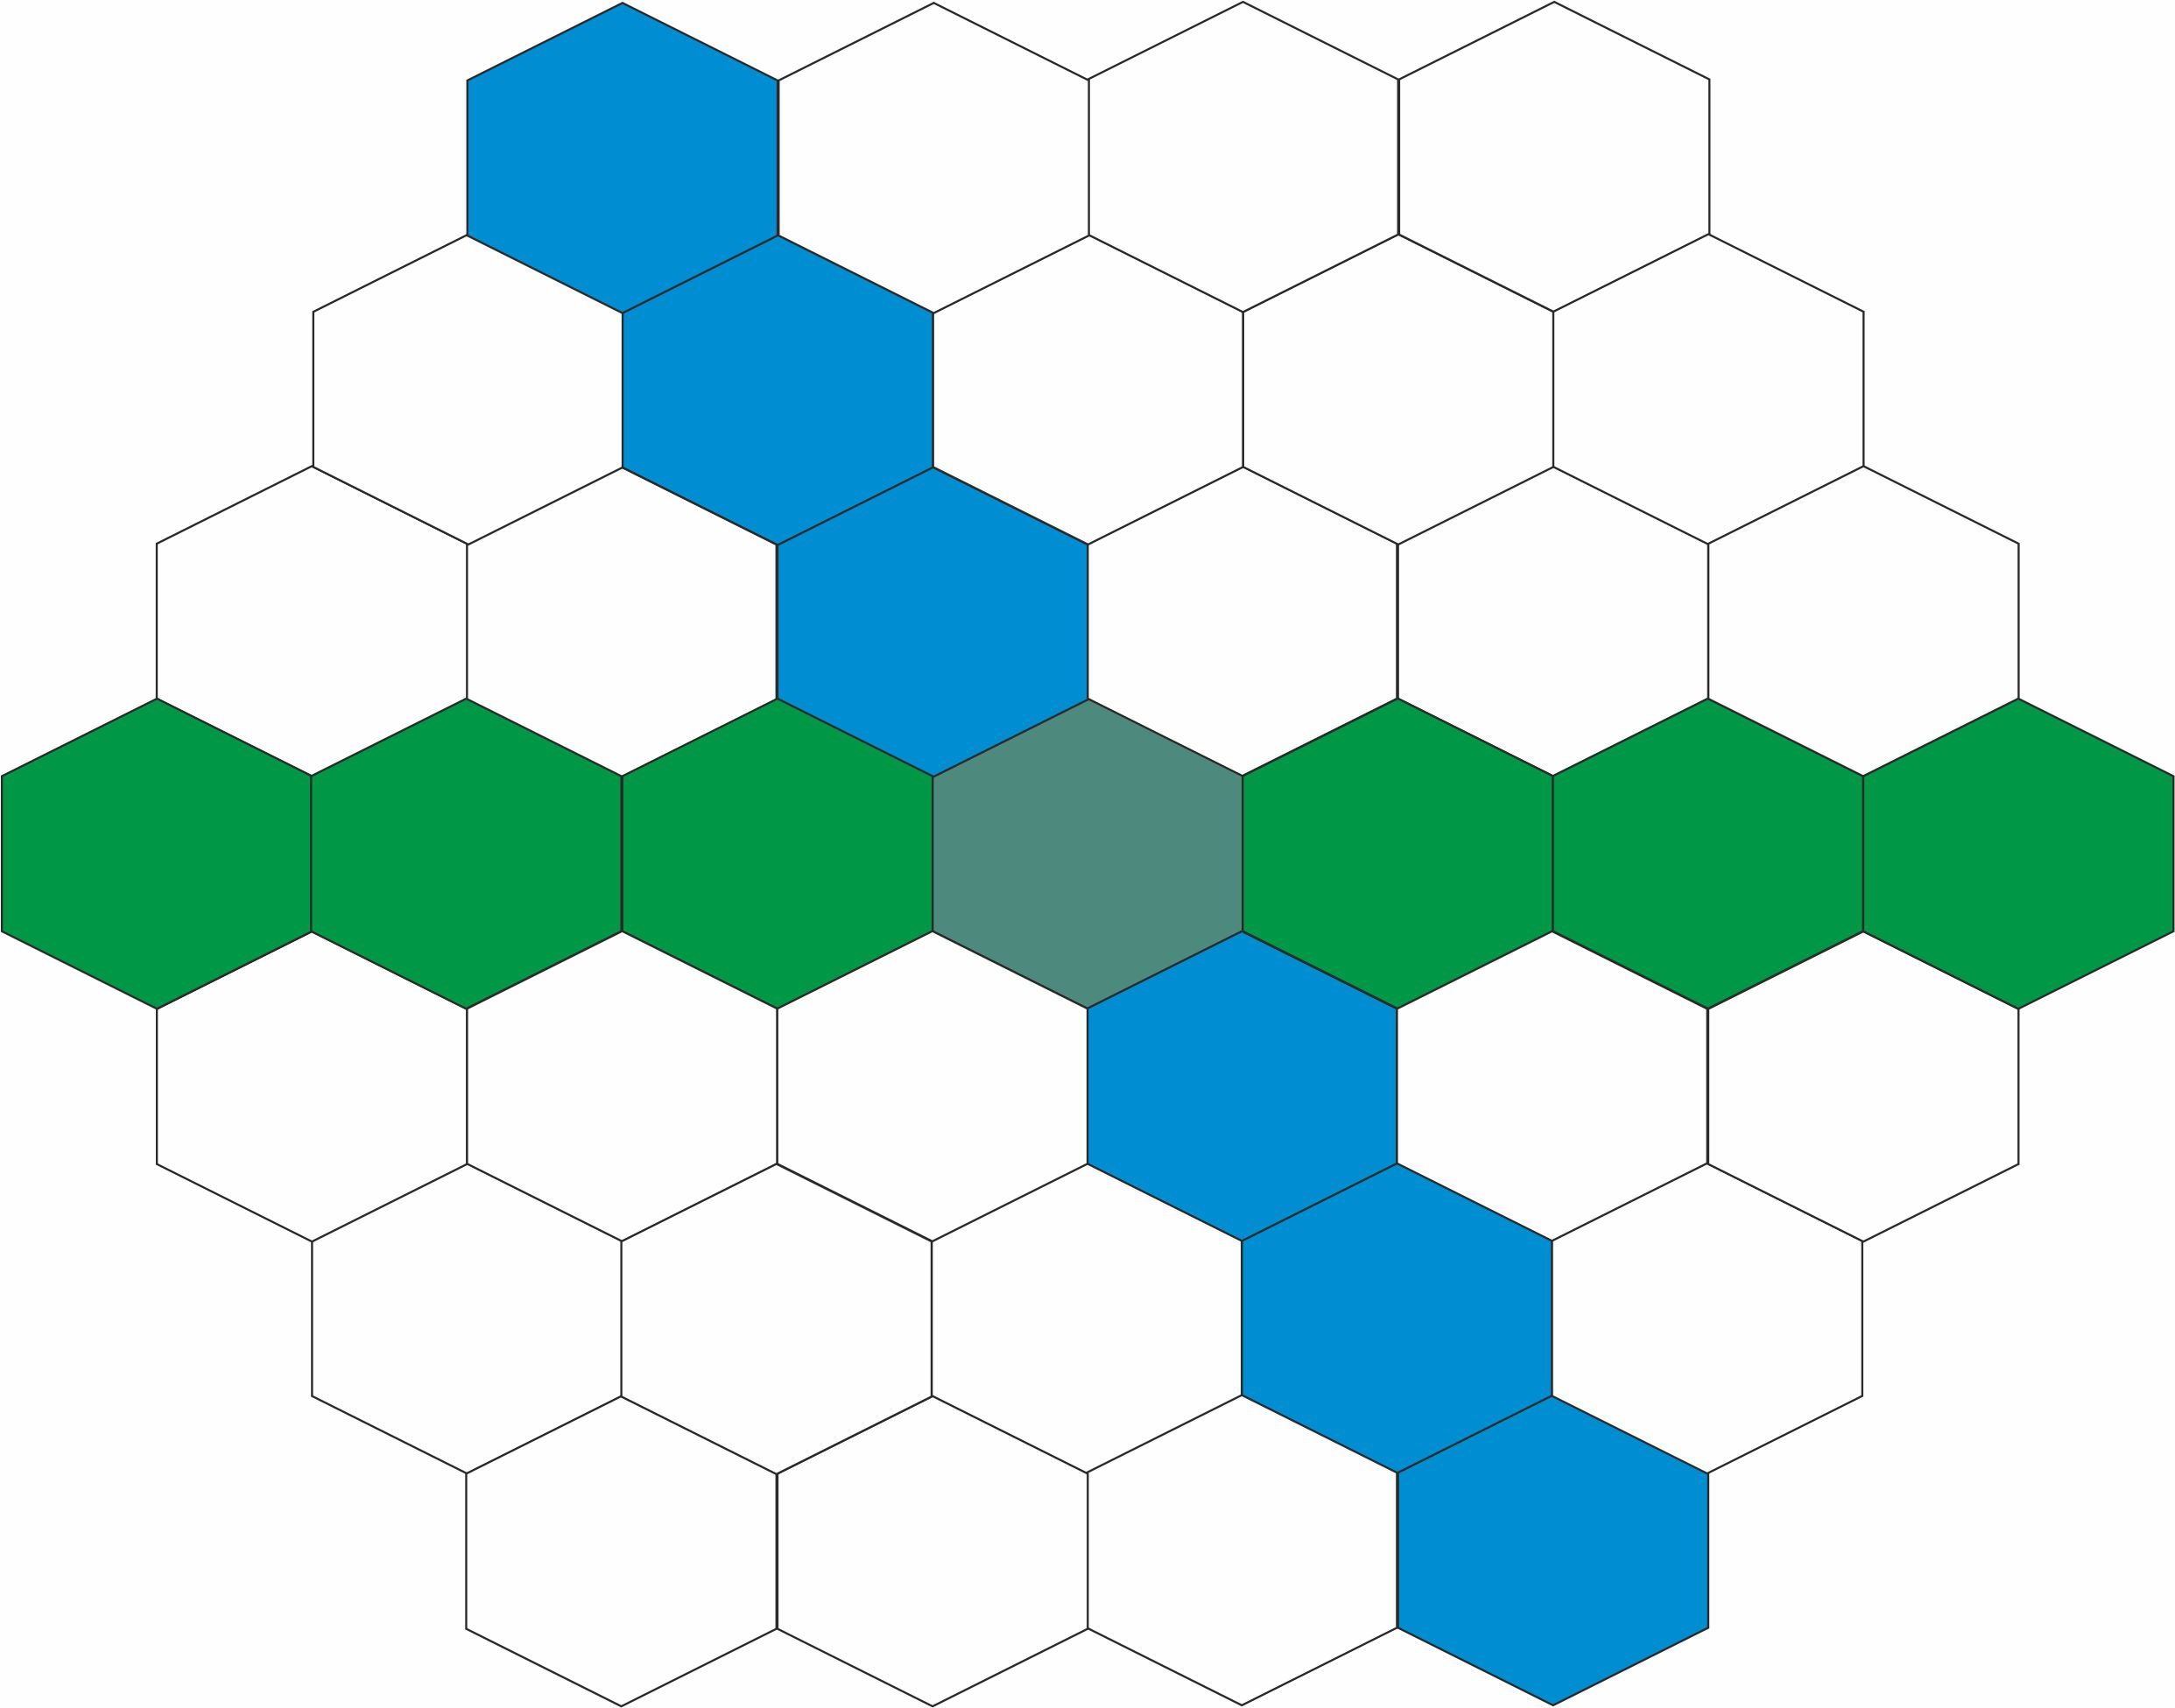
\includegraphics[scale=0.3]{kepek/AxialCoord.jpg}
\caption{A \textit{tengely koordináta-rendszer}ben a tengelyek elhelyezkedése}
\label{fig:AxialCoord}
\end{figure}

Az előnye ennek a rendszernek az eltolásoshoz képest, hogy az algoritmusok egyszerűbbek. A hátránya viszont a téglalap alakú térképek esetén való tárolás. 

\newpage
\section{Térkép tárolási probléma}
% \cite{redblobgamesHexagonalGrids}

A megjelenítő eszközeink néhány ritka kivételtől eltekintve téglalap alakúak. A számítógépes játékok jelentős része szintén téglalap alakú elrendezésekben gondolkozik. A számítógép az adatokat lineáris elrendezésben képes tárolni. A problémát az jelenti, hogy az indexeket hogyan számoljuk át úgy, hogy lehetőleg hézagmentesen tudjuk tárolni az egyes koordinátákhoz tartozó adatokat.

Síkbeli elrendezés esetén két koordináta elegendő a pozíciók egyértelmű meghatározásához. Ebből adódik, hogy a programozási nyelvekben használt mátrixos elrendezésből induljunk ki.

A következőkben annak a részletezésére kerül sor, hogy hogyan tudjuk a lehető legkevesebb kompromisszummal illeszteni a hatszög alapú elrendezésünket a kétdimenziós mátrixokhoz használt tárolási móddal.

\begin{figure}[h!]
\centering
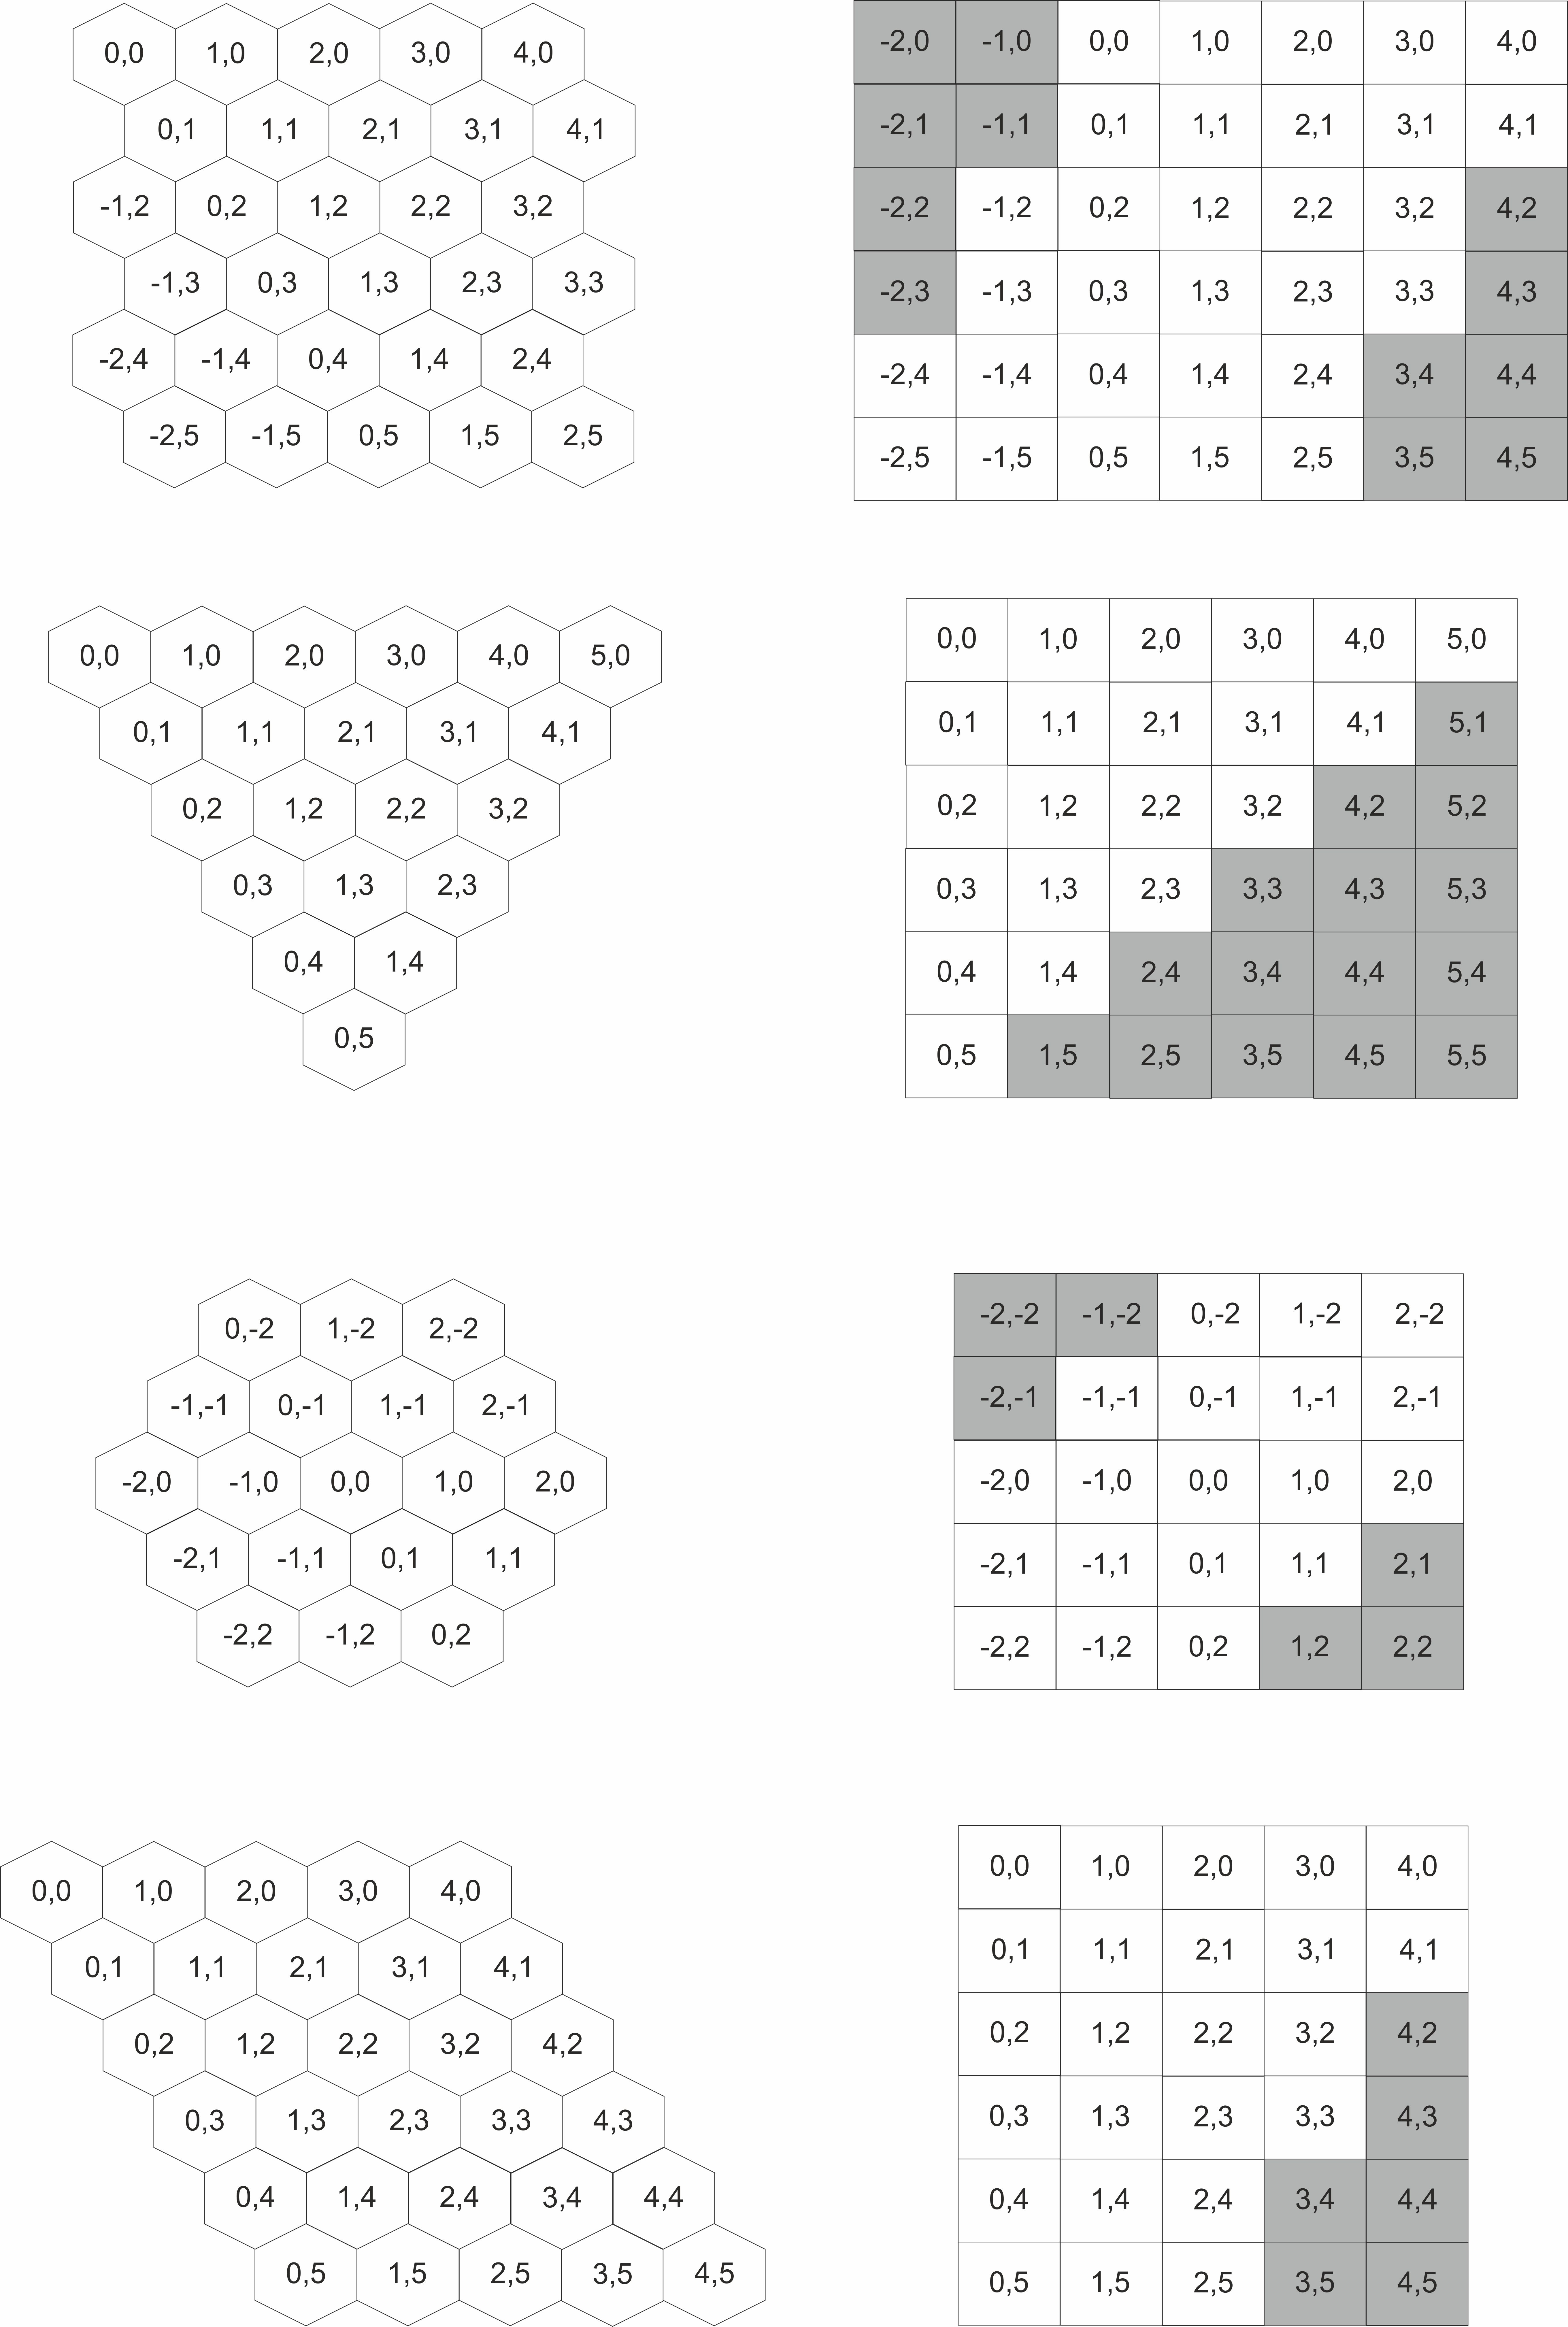
\includegraphics[scale=0.235]{kepek/StorageProblem.jpg}
\caption{Bal oldalt a különböző alakú térképek, jobb oldalt pedig a hozzájuk tárolt adat látható.}
\label{fig:StorageProblem}
\end{figure}

\noindent Vegyük észre a \ref{fig:StorageProblem}. ábrán látható képeken, hogy az elpazarolt hely a sorok bal és jobb szélén jelentkezik (kivéve a rombusz esetén). Az egyes cellákban a számpárok a $(q, r)$ oszlop és sor indexet jelölik. A hagyományos, \textit{sor-oszlop} sorrend helyett az indexelésnél az \textit{oszlop-sor} szerepel, mert a képi koordináta-rendszerekben $(x, y)$ tengely esetén ilyen sorrendben szokták használni \cite{Storage}.

Három lehetséges megoldás létezik a probléma kiküszöbölésére.
\begin{itemize}
\item Hagyjuk figyelmen kívül a problémát. Használjunk mátrixot a tárolásra és használjunk valamilyen speciális jelzőt a nem létező mezőkre. A legtöbb esetben nem éri meg ennél komplikáltabb megoldást alkalmazni.
\item Használjunk valamilyen listát a mezőkről a mátrix helyett. Ezáltal lehetőségünk lesz szabálytalan formájú térképek készítésére, beleértve azt is, hogy legyen egy lyuk a közepén. A rács osztályból \textit{getter/setter} metódusok segítségével könnyen el lehet érni (például \texttt{Grid(Tile(x, y)))}).
\item Csúsztassuk el a sorokat úgy, hogy bal oldalt ne legyen “üres” hely. Néhány nyelvben a kétdimenziós tömb az egy tömbökből álló tömb, ilyen esetekben a tömböknek nem kell egyforma hosszúaknak lenniük, így eltüntethető a felesleg a jobb oldalról is. Amennyiben egy olyan, szabálytalan alakú térképről van szó, amelynél a sorok hossza nem számítható, akkor érdemes a sorok első elemének indexeit egy külön tömbben letárolni. Ezen tömb $i$-edik elemét jelölje $a_i$. Ekkor a $q$-adik sor $r$-edik oszlopát ($0$-tól kezdődő indexet feltételezve) az $a_q + r$ címen találjuk.
\end{itemize}

Szabályos alakú térképek esetén az indexek közvetlenül számolhatók.
\begin{itemize}
\item A téglalap alakú térképek esetén az eredeti hexagonális $(q, r)$ koordinátákhoz a sorok kezdőindexeit az
$$
a_r = - \left\lfloor \dfrac{r}{2} \right\rfloor
$$
összefüggéssel számíthatjuk ki. Ez tulajdonképpen az eltolásos koordináta-rend\-szer\-be való konverziót jelenti. (A negatív index azért nem jelent problémát, mert azon $r$ értékek kerülnek levágásra, ahol az összeg negatív lenne.)
\item A háromszög alakú térképek esetén alsó- vagy felsőháromszög tárolási módot használhatunk. Alsóháromszög esetén a kezdőindexeket az
$$
a_r = \dfrac{q \cdot (q + 1)}{2}
$$
formában számíthatjuk.
\item Tekintsünk egy $N$ sugarú ($N - 1$ maximális indexekkel rendelkező) hatszög alakú térképet, ahol az origó a hatszög közepén van. Külön kell vizsgálnunk a sorindex előjelének megfelelően két esetet.

Tegyük fel, hogy $r \leq 0$. Ekkor $r$ indexű sorhoz tartozó kezdőcímet az
\begin{align*}
a_r &=
\dfrac{
(2N - 2 + r)(2N - 1 + r)
}{2}
-
\dfrac{
N(N - 1)
}{2} \\
&=
\dfrac{r^2 + (4N - 3)r + (3N^2 - 5N + 2)}{2}
\end{align*}
formában számíthatjuk ki, a címet pedig az $a_r + (N - 1 -r) + q$ alakban.

Az $r > 0$ esetben a számítást az
\begin{align*}
a_r &=
\dfrac{2N(2N - 1)}{2} -
\dfrac{(2N - r - 1)(2N - r)}{2} +
\dfrac{(2N - 1)(2N - 2)}{2} -
\dfrac{N(N - 1)}{2} \\
&=
\dfrac{-r^2 + (4N - 1)r + (3N^2 - 5N + 2)}
{2}
\end{align*}
összefüggés írja le. A $(q, r)$ koordinátájú elem indexe ekkor $a_r + (N - 1 + r) + q$ értékével lesz egyenlő.
\item A rombusz formájú térkép esetén minden tökéletesen egyezik, ezért egyszerűen csak az $a_r = 0$ kezdőindexekkel kell számolnunk.
\end{itemize}

\section{Koordináta konverziók}

Mivel a három terület ahol a koordinátákat használjuk (tárolás, megjelenítés, számítások) nem feltétlenül ugyanabban a koordináta-rendszerben fognak megvalósulni, ezért szükséges ismernünk a különböző konverziós eljárásokat oda-vissza a különböző rendszerek között. Mivel a számításokhoz a \textit{kocka koordináta-rendszer}t fogom alkalmazni, ezért erre a rendszerre fogom alapozni az algoritmusokat \cite{Conversion}.

\subsection{Tengely - Kocka konverziók}
% \cite{redblobgamesHexagonalGrids}

A \textit{tengely koordináta-rendszer} nagyon közel áll a \textit{kocka koordináta-rendszer}hez. A tengelyes csak elhagyja a harmadik koordinátát, a kocka pedig kiszámolja a harmadikat a másik kettő alapján \cite{Conv_Axial}.

%\begin{verbatim}
%function cube_to_axial(cube):
%    var q = cube.x
%    var r = cube.z
%    return Hex(q, r)
%function axial_to_cube(hex):
%    var x = hex.q
%    var z = hex.r
%    var y = -x-z
%    return Cube(x, y, z)
%\end{verbatim}

\begin{align*}
axial_{q, r}(cube_{x}, cube_{y}) &=
\left(
\begin{array}{c}
cube_{x} \\
cube_{y}
\end{array}
\right)
\\
cube_{x,y,z} (axial_{q}, axial_{r}) &=
\left(
\begin{array}{c}
axial_q \\
axial_r \\
-axial_q - axial_r
\end{array}
\right)
\end{align*}

\subsection{Eltolásos - Kocka konverziók}
% \cite{redblobgamesHexagonalGrids}

Az \textit{eltolásos koordináta-rendszer}nek négy fajta típusa lehet az alapján, hogy melyik sor/oszlop lett eltolva. A páratlan indexű sorok eltolása esetén a következő formában számítható az összefüggés \cite{Conv_Offset}.
\begin{align*}
&oddrow_{row, col}(cube_{x},cube_{z}, cube_{z}) =
\left(
\begin{array}{c}
cube_{x} + \dfrac{cube_{z} - (cube_{z} \bmod 2)}{2} \\
cube_{z}
\end{array}
\right),
\\
&cube_{x, y, z}(oddrow_{row}, oddrow_{col}) =
\left(
\begin{array}{c}
oddrow_{col} - \dfrac{oddrow_{row} - (oddrow_{row} \bmod 2)}{2} \\
oddrow_{row} \\
-cube_{x} - cube_{y}
\end{array}
\right)
\end{align*}

%\begin{verbatim}
%function cube_to_oddr(cube):
%      col = cube.x + (cube.z - (cube.z&1)) / 2
%      row = cube.z
%      return Hex(col, row)
%
%function oddr_to_cube(hex):
%      x = hex.col - (hex.row - (hex.row&1)) / 2
%      z = hex.row
%      y = -x-z
%      return Cube(x, y, z)
%\end{verbatim}

A páros indexű sorok eltolása esetén a következő módon számíthatjuk az indexeket.
\begin{align*}
&evenrow_{row, col}(cube_{x}, cube_{z}) =
\left(
\begin{array}{c}
cube_{z} \\
cube_{x} + \dfrac{cube_{z} + (cube_{z} \bmod 2)}{2} \\
\end{array}
\right),
\\
&cube_{x, y, z}(evenrow_{row}, evenrow_{col}) = \\
&\left(
\begin{array}{c}
evenrow_{col} - \dfrac{evenrow_{row} + (evenrow_{row} \bmod 2)}{2} \\
-cube_{x} - cube_{z} \\
evenrow_{row} \\
\end{array}
\right)
\end{align*}


%\begin{verbatim}
%function cube_to_evenr(cube):
%      col = cube.x + (cube.z + (cube.z&1)) / 2
%      row = cube.z
%      return Hex(col, row)
%
%function evenr_to_cube(hex):
%      x = hex.col - (hex.row + (hex.row&1)) / 2
%      z = hex.row
%      y = -x-z
%      return Cube(x, y, z)
%\end{verbatim}

Páratlan indexű oszlop eltolásakor a számítás:

\begin{align*}
&oddcolumn_{row, col}(cube_{x}, cube_{z}) =
\left(
\begin{array}{c}
cube_{z} + \frac{cube_{x} - (cube_{x} \bmod 2)}{2} \\
cube_{x} \\
\end{array}
\right),
\\
&cube_{x,y,z} (oddcolumn_{row}, oddcolumn_{col}) = \\
&\left(
\begin{array}{c}
oddcolumn_{col} \\
-cube_{x} - cube_{z} \\
oddcolumn_{row} - \dfrac{oddcolumn_{col} - (oddcolumn_{col} \bmod 2)}{2} \\
\end{array}
\right).
\end{align*}

%\begin{verbatim}
%function cube_to_oddq(cube):
%      col = cube.x
%      row = cube.z + (cube.x - (cube.x&1)) / 2
%      return Hex(col, row)
%
%function oddq_to_cube(hex):
%      x = hex.col
%      z = hex.row - (hex.col - (hex.col&1)) / 2
%      y = -x-z
%      return Cube(x, y, z)
%\end{verbatim}

Utolsó esetként a páros indexű oszlopokkal való eltolás számítása a következő:

\begin{align*}
&evencolumn_{row, col}(cube_{x}, cube_{z}) =
\left(
\begin{array}{c}
cube_{z} + \frac{cube_{x} + (cube_{x} \bmod 2)}{2} \\
cube_{x} \\
\end{array}
\right),
\\
&cube_{x,y,z}(evencolumn_{row}, evencolumn_{col}) = \\
&\left(
\begin{array}{c}
evencolumn_{col} \\
-cube_{x} - cube_{z} \\
evencolumn_{row} - \dfrac{evencolumn_{col} + (evencolumn_{col} \bmod 2)}{2}
\end{array}
\right).
\end{align*}

%\begin{verbatim}
%function cube_to_evenq(cube):
%      col = cube.x
%      row = cube.z + (cube.x + (cube.x&1)) / 2
%      return Hex(col, row)
%
%function evenq_to_cube(hex):
%      x = hex.col
%      z = hex.row - (hex.col + (hex.col&1)) / 2
%      y = -x-z
%      return Cube(x, y, z)
%\end{verbatim}

Az implementációban érdemes \textit{bitenkénti “és”} (\texttt{a \& 1}) operátort használni \textit{modulo} (\texttt{a \% 2}) helyett, amikor meghatározzuk, hogy páros vagy páratlan sorban/oszlopban vagyunk, mivel ez működik negatív számok esetén is, függetlenül a maradékképzés műveletének programnyelvi implementálási módjától.

\newpage
\section{Távolságok számítása}
\label{sec:tavolsag}

Ahhoz, hogy távolságokat tudjunk számolni a térképen definiálnunk kell hozzá metrikákat. A különböző típusú koordináta-rendszerek esetén ennek különféle módjai lehetnek. A következő szakaszok ezek közül mutatnak be néhányat \cite{Distance}.

\subsection{Kocka koordináta-rendszer}
% \cite{redblobgamesHexagonalGrids}

A \textit{kocka koordináta-rendszer}ben, minden hexagon egy kockának felel meg a három dimenziós térben. A szomszédos hexagonok 1 távolságra vannak egymástól a hexagonháló esetén, viszont 2 távolságra vannak egymástól a \textit{kocka koordináta-rendszer}ben. Ezáltal egyszerűbbé válik a távolságszámítás.

Jelölje $dx$ az $x$ tengely irányú különbségeket, a $dy$ és $dz$ pedig hasonlóképp az $y$ és $z$ tengelyek esetében. A \textit{négyzet koordináta-rendszer} esetén a \textit{Manhattan-távolság} távolság az $|dx| + |dy|$ formában írható föl. Ugyanez \textit{kocka koordináta-rendszer}ben $|dx| + |dy| + |dz|$. Ezekből következik, hogy a hexagonrács esetén a \textit{Manhattan-távolság} a kockarács esetén fennálló távolság fele, vagyis
$$
d_{\text{cube}}(a, b) =
\dfrac{|a_x - b_x| + |a_y - b_y| + |a_z - b_z|}{2}.
$$

Egy ezzel egyenértékű megközelítés az is, ha megfigyeljük azt, hogy a három koordináta közül az egyiknek mindenképpen a másik kettő összegének kell lennie. Ekkor az az egy lesz a távolság \cite{Distance_Cube}:
$$
d_{\text{cube}}(a, b) =
\max(
|a_x - b_x|, |a_y - b_y|, |a_z - b_z|
).
$$

\subsection{Tengelyes koordináta-rendszer}
%\cite{redblobgamesHexagonalGrids}
%\cite{HexagonalGrids}

A \textit{tengelyes koordináta-rendszer}ben a számításokhoz szükséges három koordinátából kettőt ismerünk, ezért konvertálnunk kell majd a \textit{kocka koordináta-rendszer}re \cite{Distance_Axial}:
$$
d_{hex}(a, b) = \frac{|a_x - b_x| + |a_x + a_y - b_x - b_y| + |a_z - b_z|}{2}.
$$

\subsection{Eltolásos koordináta-rendszer}
%\cite{redblobgamesHexagonalGrids}
%\cite{HexagonalGrids}

Az \textit{eltolásos koordináta-rendszer} esetén azt a megoldást fogjuk használni, hogy átalakítjuk a koordinátákat a \textit{kocka koordináta-rendszer}re, vagyis \cite{Distance_Offset}
$$
d_{of\!fset} (a, b) = d_{cube}(cube_a, cube_b).
$$

